\section{Kubernetes}

\sectionslide{Kubernetes}
\begin{frame}
	\frametitle{Scaling applications / services}
	\begin{columns}[t]
		\column{.3\textwidth}
		\hervor{Monolithic Architecture}
		
		\textit{\footnotesize "Our applications run on one server (e.g. webserver and database). If you need to update, you have to power the whole system down."}

		\column{.3\textwidth}
		\hervor{Containerized architecture}
		
		\textit{\footnotesize "We test our applications and ship them to our production server(s) with all dependencies. On update, downtime is really small."}


		\column{.4\textwidth}
		\hervor{Distributed, managed architecture}
		
		\textit{\footnotesize "Our applications consist of independent microservices that communicate via interfaces, they can be replaced / updated without downtime. The system itself dynamically adapts to workload by scaling up/down."}

	\end{columns}

	\begin{columns}
		\column{.3\textwidth}
		\centering
		\resizebox{\textwidth}{!}{
			\begin{tikzpicture}
				\node[] (serv) at (0,0) {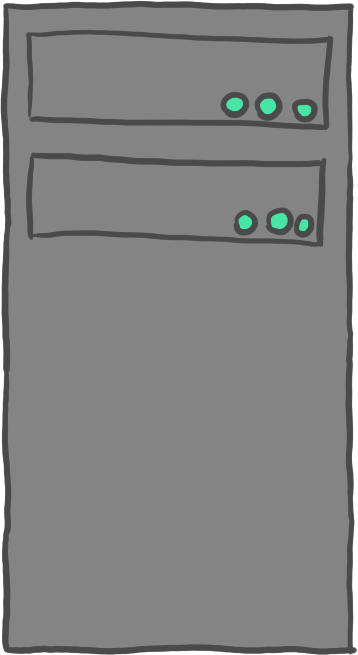
\includegraphics[width=1.7cm]{pics/server.png}};
				\node[] (pl) [right=-0.2cm of serv] {\Huge +};
				\node[] (apps) [right=-0.2cm of pl] {
\includegraphics[width=1.7cm]{pics/apps.png}};
		\end{tikzpicture}}
		
		\column{.3\textwidth}
		\centering
		\resizebox{\textwidth}{!}{
			\begin{tikzpicture}
				\node[anchor=north west] (serv1) at (0,0) {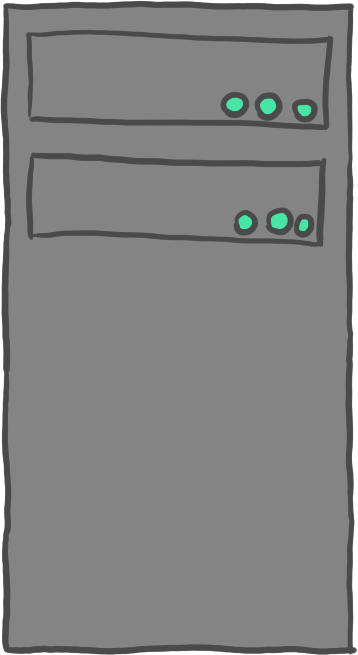
\includegraphics[width=1.7cm]{pics/server.png}};
				
				\node[anchor=north west] (pl) [right=-0.2cm of serv1]  {\Huge +};
				\node[] (c1) [right=-0.2cm of pl] {
\includegraphics[width=2.3cm]{pics/container_large_no_write.png}};
				\node[] (c2) [below=-0.1cm of c1] {
\includegraphics[width=2.3cm]{pics/container_large_no_write.png}};
				\node[] (c3) [above=-0.1cm of c1] {
\includegraphics[width=2.3cm]{pics/container_large_no_write.png}};
			\end{tikzpicture}
		}
		
		\column{.4\textwidth}
		\centering
		\resizebox{.8\textwidth}{!}{
			\begin{tikzpicture}
				\node[anchor=north west] (serv1) at (0,0) {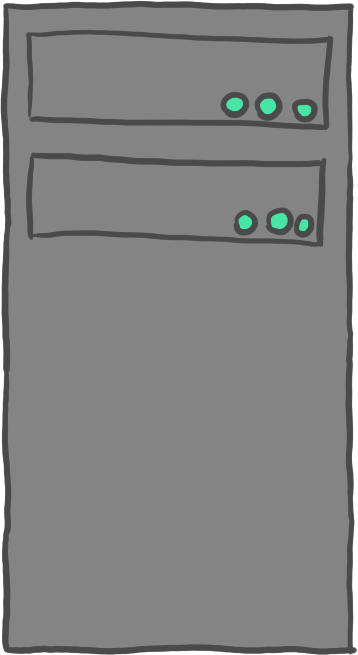
\includegraphics[width=0.62cm]{pics/server.png}};
				\node[anchor=north west] (serv2) [below=-0.2cm of serv1] {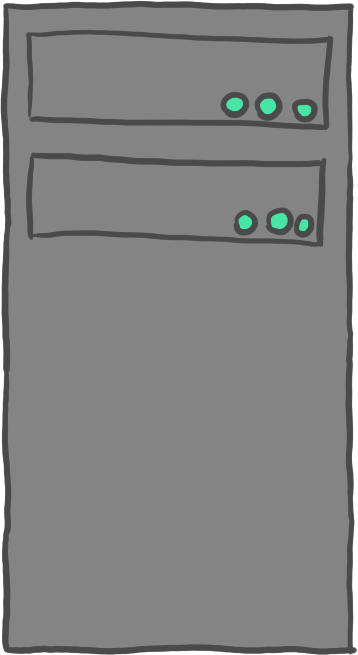
\includegraphics[width=0.62cm]{pics/server.png}};
				\node[anchor=north west] (serv3) [above=-0.2cm of serv1] {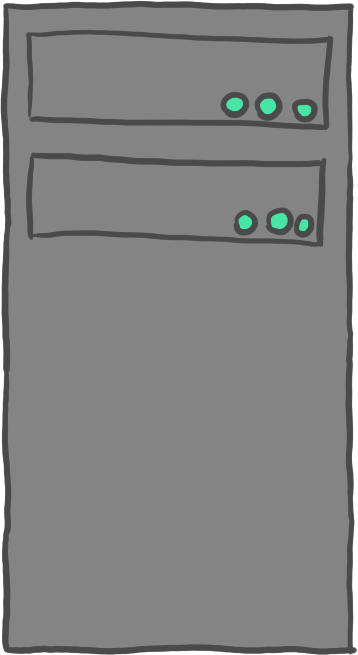
\includegraphics[width=0.62cm]{pics/server.png}};
				\node[anchor=north west] (serv4) [left=-0.2cm of serv1] {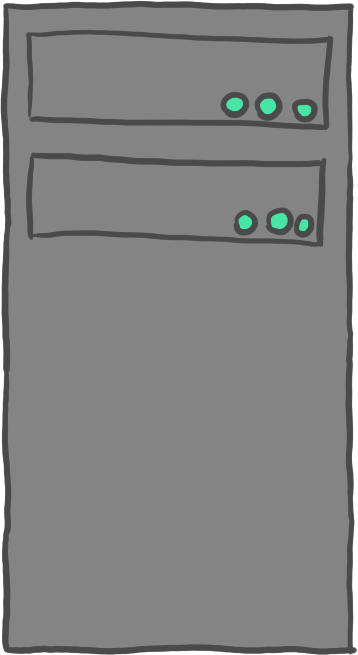
\includegraphics[width=0.62cm]{pics/server.png}};
				\node[anchor=north west] (serv5) [below=-0.2cm of serv4] {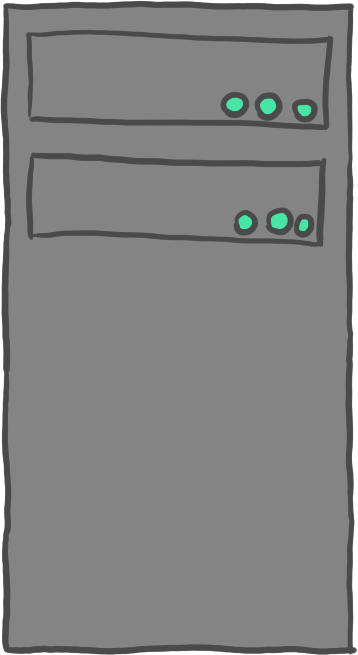
\includegraphics[width=0.62cm]{pics/server.png}};
				\node[anchor=north west] (serv6) [above=-0.2cm of serv4] {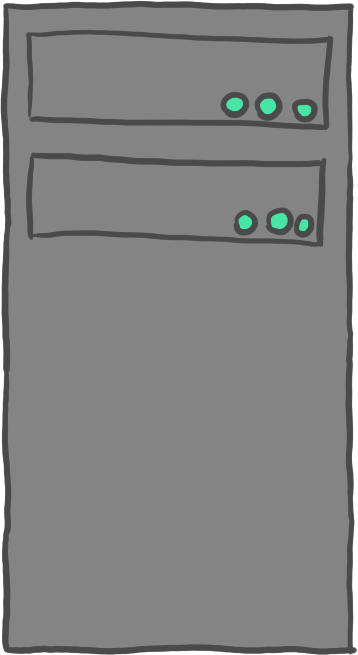
\includegraphics[width=0.62cm]{pics/server.png}};
				\node[anchor=north west] (serv7) [left=-0.2cm of serv4] {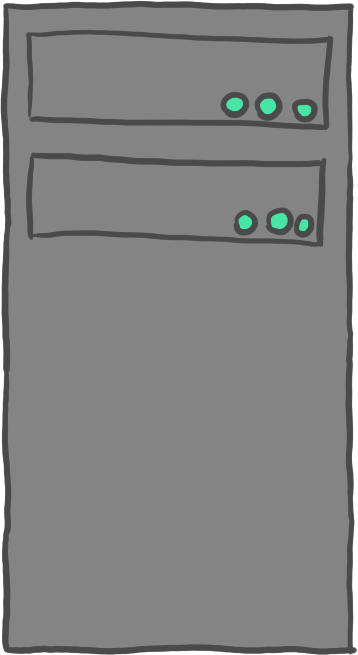
\includegraphics[width=0.62cm]{pics/server.png}};
				\node[anchor=north west] (serv8) [below=-0.2cm of serv7] {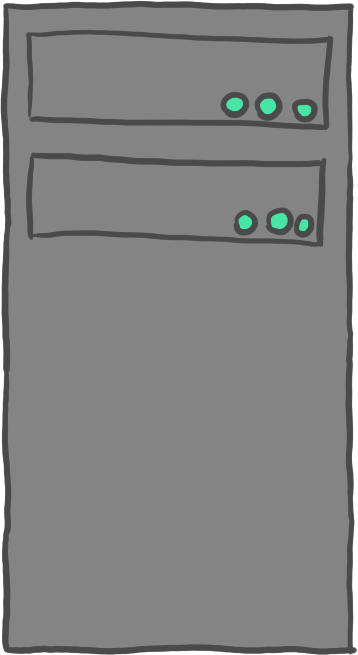
\includegraphics[width=0.62cm]{pics/server.png}};
				\node[anchor=north west] (serv9) [above=-0.2cm of serv7] {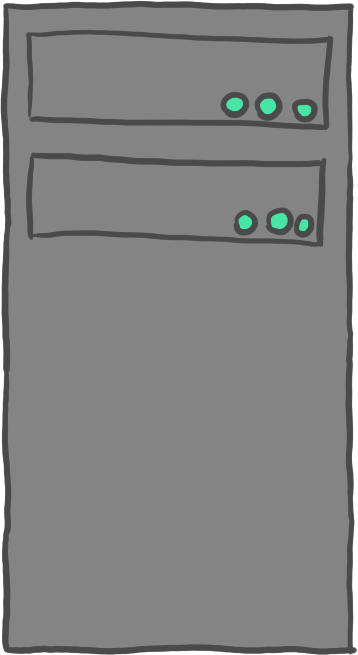
\includegraphics[width=0.62cm]{pics/server.png}};
				\node[anchor=north west] (pl) [right=-0.2cm of serv1]  {\Huge +};
				\node[] (c1) [right=-0.2cm of pl] {
\includegraphics[width=1.9cm]{pics/container_large_no_write.png}};
				\node[] (c2) [below=-0.2cm of c1] {
\includegraphics[width=1.9cm]{pics/container_large_no_write.png}};
				\node[] (c3) [above=-0.2cm of c1] {
\includegraphics[width=1.9cm]{pics/container_large_no_write.png}};
				\node[] (c4) [above=-0.2cm of c3] {
\includegraphics[width=1.9cm]{pics/container_large_no_write.png}};
				\node[] (c5) [below=-0.2cm of c2] {
\includegraphics[width=1.9cm]{pics/container_large_no_write.png}};
		\end{tikzpicture}}
	\end{columns}
\end{frame}

\begin{frame}
	\frametitle{Kubernetes}
	\vspace{-.1cm}\begin{block}{Kubernetes (K8s) according to the \myhref{https://kubernetes.io/docs/concepts/overview/what-is-kubernetes/}{documentation:}}
		\begin{columns}
			\column{.15\textwidth}
			\centering
			\vspace{.1cm}\\
			
\includegraphics[width=.75\textwidth]{pics/kubernetes_logo.png}
			
			\column{.85\textwidth}
			"Kubernetes is a portable, extensible, open-source platform for managing containerized workloads and services, that facilitates both declarative configuration and automation."
		\end{columns}
	\end{block}
	\centering
	\vspace{-.1cm}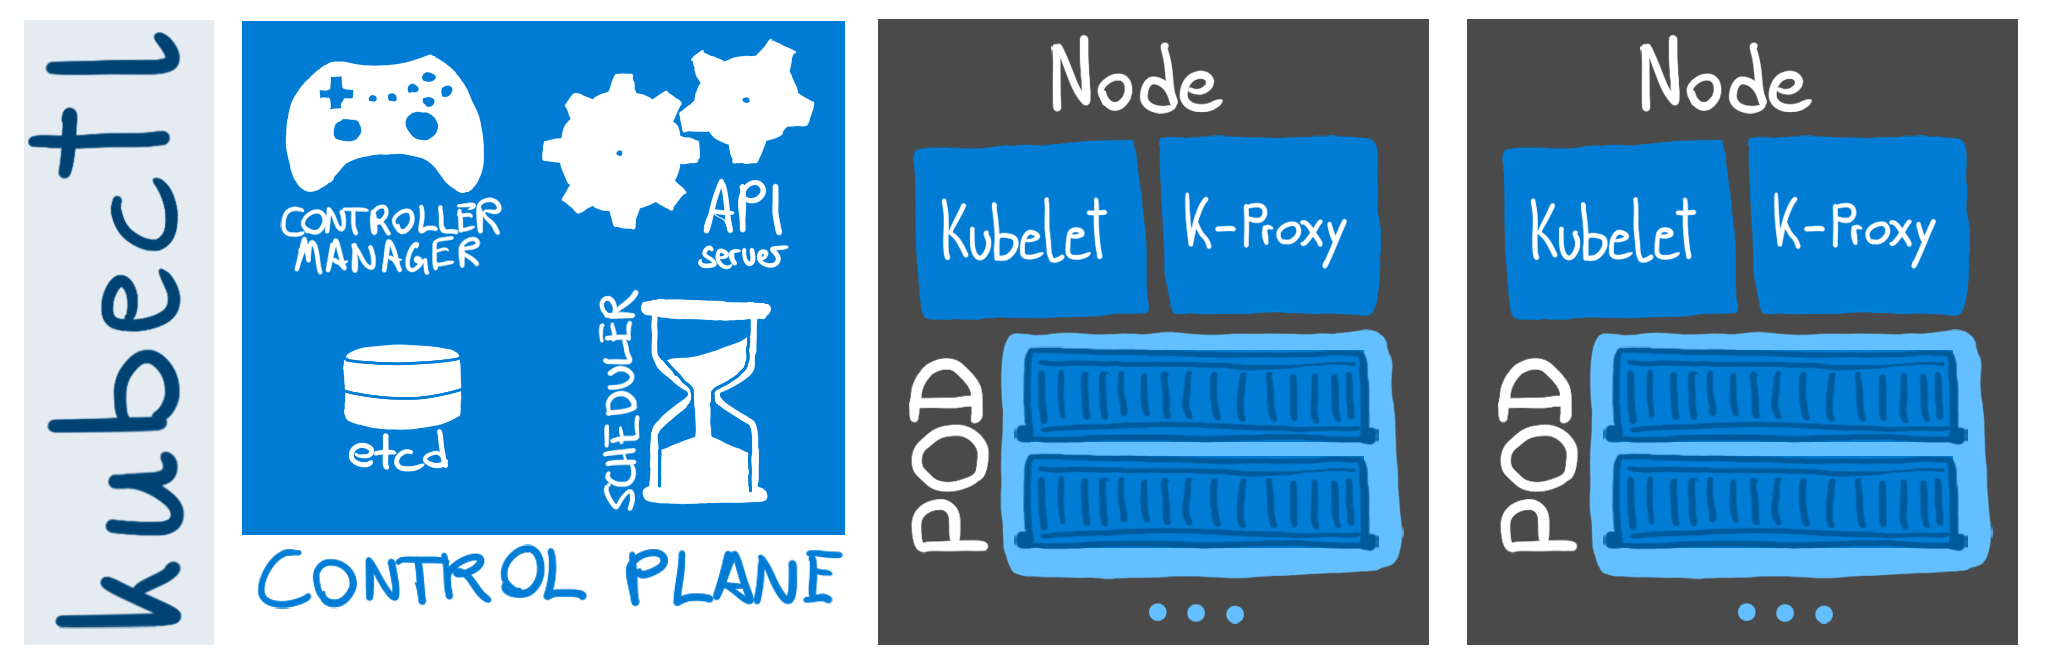
\includegraphics[width=\textwidth]{pics/kubernetes_sketch.png}
\end{frame}

\begin{frame}[fragile]
	\frametitle{Kubernetes objects}
		Just a few should be mentioned here:
		\begin{itemize}
			\item \hervor{Deployment}: packaged application consisting of several containers run in a \hervor{Pod}. Can be replicated for load balancing.
			\item  \hervor{Service}: A connection to an application, "pod-agnostic" for availability
			\item \hervor{Pods}, \hervor{Nodes}, etc. are Kubernetes objects too! Get information about them with
			\begin{lstlisting}
# info for all objects of one type
kubectl get object
kubectl describe object
# info for a specific object
kubectl get object objectname
kubectl describe object objectname
			\end{lstlisting}
		\item \hervor{Control Plane} controls a cluster of \hervor{Nodes}
		\item containers are deployed in \hervor{Pods} on \hervor{Nodes}
			\end{itemize}

\end{frame}

\begin{frame}[fragile]
	\frametitle{Interacting with the cluster: \texttt{kubectl}}
	\begin{block}{\texttt{kubectl}}
	is a CLI tool to send commands to the \hervor{API server} for creating Kubernetes objects.
	\end{block}
	\codi{kubectl} creates objects
	\begin{itemize}
		\item \hervor{imperatively}: Everything explicitly on the command line 
		\item \hervor{declaratively}: with a \hervor{spec} representing the desired state (\codi{.yaml}-file)
	\end{itemize}
	Let the cluster work to realize your spec:
	\begin{lstlisting}
kubectl apply -f kubernetes/greeting-depl-0-1.yaml
kubectl apply -f kubernetes/greeting-depl-0-2.yaml
	\end{lstlisting}
	Declarative way is preferred and more practicable!
\end{frame}

\begin{frame}[fragile]
	\frametitle{Create a greeting app deployment and service}
	\vspace{-.2cm}\begin{columns}
		\column{.5\textwidth}
		\begin{lstlisting}
apiVersion: apps/v1
kind: Deployment
metadata:
  name: greeting-depl
spec:
  selector:
	matchLabels:
	  app: greetingapp
  replicas: 2 # 2 pods of template
  template:
	metadata:
	  labels:
		app: greetingapp
	spec:
	  containers:
	  - name: greet
		image: greeting:0.1
		ports:
		- containerPort: 5000
		\end{lstlisting}
	
		\column{.47\textwidth}
		\textbf{Example:} \codi{kubernetes/greeting-depl-0-1.yaml}
		\begin{lstlisting}
kubectl apply \
	-f greeting-depl-0-1.yaml
# see what just happened
kubectl get deployments
kubectl get pods
kubectl logs podname containername
		\end{lstlisting}

		Make available by creating a \hervor{service}:
		\begin{lstlisting}
kubectl expose deployment \
	greeting-depl \
	--type=NodePort \
	--port 5000
# note the port it gets mapped to
kubectl get services
# run proxy for access on localhost
kubectl proxy
		\end{lstlisting}
	\end{columns}
\end{frame}

\begin{frame}[fragile]
	\frametitle{Update greeting app deployment}

		\textbf{Example:} \codi{kubernetes/greeting-depl-0-2.yaml}
		\begin{itemize}
			\item Updated greeting image version
			\item Added postgres container
		\end{itemize}
		Declare the new spec:
		\begin{lstlisting}
kubectl apply -f greeting-depl-0-2.yaml
		\end{lstlisting}
	\begin{itemize}
		\item Pods are replaced one by one, without the service terminating!
		\item Eventually, you will see the newer greeting app.
		\end{itemize}
		
		Tidy up:
		\begin{lstlisting}
kubectl delete service greeting-depl
kubectl delete deployment greeting-depl
		\end{lstlisting}
		Containers and pods are terminated!
		
	
\end{frame}

\begin{frame}
	\frametitle{Concluding notes}
	
	\begin{itemize}
		\item replicas $>1$: we do not know which of our apps we will get (\hervor{load balancing}, no persistent storage)
		\item persistent storage is possible, here only stateless applications were shown
		\item \textbf{Not mentioned here:} security, encryption, secrets
		\item Docker Desktop users can activate a one-node kubernetes cluster in the settings
		\item Another one-node try-out solution: \myhref{https://minikube.sigs.k8s.io/docs/}{Minikube}
	\end{itemize}

	\begin{block}{Further reading:}
	\begin{itemize}
		\item \myhref{https://kubernetes.io/docs/home/}{Kubernetes documentation}: Includes lots of learning resources and examples.
		\item \myhref{https://training.play-with-kubernetes.com/}{Play with Kubernetes classroom}: Interactive training session giving an overview over concepts.
	\end{itemize}
	
	\end{block}
\end{frame}